\documentclass[11pt]{article}
\usepackage[a4paper,margin=1in]{geometry}
\usepackage{amsmath,amssymb,amsthm}
\usepackage{tikz}
\usetikzlibrary{arrows.meta,calc,decorations.pathreplacing}
\usepackage{xcolor}
\usepackage{booktabs}
\usepackage[hidelinks]{hyperref}
\hypersetup{pdftitle={A broken stick and a Feynman diagram},pdfauthor={Vamshi Jandhyala}}
\setlength{\parskip}{0.4em}
\setlength{\parindent}{0pt}

\newtheorem{theorem}{Theorem}
\newtheorem{lemma}{Lemma}
\newtheorem{corollary}{Corollary}
\theoremstyle{remark}
\newtheorem*{remark}{Remark}

\definecolor{inkblue}{RGB}{40,76,105}
\definecolor{softblue}{RGB}{226,235,243}
\definecolor{rust}{RGB}{153,70,45}

\newcommand{\R}{\mathbb{R}}
\newcommand{\dd}{\mathrm{d}}
\newcommand{\abs}[1]{\left|#1\right|}

\title{A broken stick and a Feynman diagram}
\author{Vamshi Jandhyala}
\date{}

\begin{document}
\maketitle
\vspace{-2em}

\begin{abstract}
Break a stick at five random points and use the six pieces, in a fixed order, as the edges of a
tetrahedron. How often does a tetrahedron exist? We show that the answer is a Feynman integral: up to an
explicit constant it is the three-loop tetrahedron vacuum diagram in four dimensions, with equal masses
and every propagator raised to the power $3/2$. The same argument works in every dimension, with the
complete graph $K_{n+1}$ in place of the tetrahedron, and for $n=2$ it gives the classical answer $1/4$ for
triangles. Two independent computations of the tetrahedron integral agree to within $10^{-12}$, giving
$0.0125749944167\ldots$, which corrects a value of $1/79$ reported from simulation. The algebraic steps are
checked in the Lean proof assistant.
\end{abstract}

\section{Six pieces of a stick}

Take a stick of length $1$ and break it at five points chosen independently and uniformly at random.
Label the six pieces in order along the stick and lay them on the six edges of a tetrahedron in a fixed
way, as in Figure~\ref{fig:stick}. Write $p_3$ for the probability that some tetrahedron in space has
exactly these edge lengths.

\begin{figure}[ht]
\centering
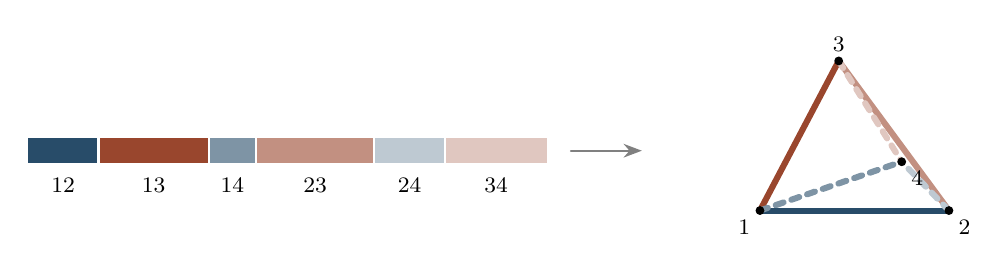
\begin{tikzpicture}[scale=1.0,line cap=round]
  % the stick, cut at five points (lengths drawn to scale for one sample)
  \def\cuts{0,0.9,2.3,2.9,4.4,5.3,6.6}
  \foreach \a/\b/\lab/\c in {0/0.9/12/inkblue,0.9/2.3/13/rust,2.3/2.9/14/inkblue!60,2.9/4.4/23/rust!60,4.4/5.3/24/inkblue!30,5.3/6.6/34/rust!30}{
    \fill[\c] (\a,0) rectangle (\b,0.32);
    \node[font=\footnotesize] at ({(\a+\b)/2},-0.28) {$\lab$};
  }
  \foreach \x in {0.9,2.3,2.9,4.4,5.3}{\draw[thick,white] (\x,-0.02) -- (\x,0.34);}
  \draw[->,>=Stealth,thick,gray] (6.9,0.16) -- (7.8,0.16);
  % the tetrahedron, edges coloured as the pieces
  \begin{scope}[shift={(9.3,-0.6)}]
    \coordinate (1) at (0,0); \coordinate (2) at (2.4,0); \coordinate (3) at (1.0,1.9); \coordinate (4) at (1.8,0.62);
    \draw[line width=2.2pt,inkblue] (1) -- (2);
    \draw[line width=2.2pt,rust] (1) -- (3);
    \draw[line width=2.2pt,inkblue!60,dashed] (1) -- (4);
    \draw[line width=2.2pt,rust!60] (2) -- (3);
    \draw[line width=2.2pt,inkblue!30,dashed] (2) -- (4);
    \draw[line width=2.2pt,rust!30,dashed] (3) -- (4);
    \foreach \p/\pos in {1/below left,2/below right,3/above,4/below right}{\fill (\p) circle (1.6pt); \node[\pos,font=\footnotesize] at (\p) {$\p$};}
  \end{scope}
\end{tikzpicture}

\caption{A stick broken at five random points. The pieces go to fixed edges of a tetrahedron, here
$12,13,14,23,24,34$ in order. The question is whether a tetrahedron with these edge lengths exists.}
\label{fig:stick}
\end{figure}

The one-dimension-lower version is a classic. Stop and try it before reading on: break a stick at two
random points; how likely are the three pieces to form a triangle? The answer is $1/4$, because the
triangle exists exactly when no piece is longer than $1/2$, and each of the three ways to fail cuts off
a quarter of the triangle of possible lengths.

For the tetrahedron the four faces must satisfy the triangle inequality, but that is not enough. Douglas
Zare observed on MathOverflow that the twelve triangle inequalities cut out a polytope with $1/54$ of the
possible lengths~\cite{Zare}. Inside it a sixth-degree polynomial in the lengths, the Cayley--Menger
determinant, must also have the right sign, and this extra condition removes about a third of the
polytope. Benjamin Dickman asked the question in 2013~\cite{MO,MSE}, and surveys of broken-stick
problems pose it as the natural next case~\cite{IP10,Ver22}. No exact value has been found, and the only numbers so far are numerical
estimates, one of which, $1/79$, is reported in the comments of~\cite{MO}.

This note does not find a closed form either. It shows instead why the number is hard, by identifying it
with an object physicists have studied for decades. Write $N=n(n+1)/2$ for the number of edges of an
$n$-simplex and $U$ for the first Symanzik polynomial of the complete graph $K_{n+1}$ (defined in
Section~\ref{sec:tree}): for each spanning tree, multiply the variables of the edges \emph{not} in the
tree, and add over all spanning trees. Let $p_n$ be the probability that $N$ pieces of a randomly broken
stick, laid on the edges of an $n$-simplex in a fixed order, are its edge lengths.

\begin{theorem}\label{thm:main}
For every $n\ge 2$,
\begin{equation}\label{eq:main}
p_n=C_n\int_{\R_+^N}\frac{\prod_e \beta_e^{(n-2)/2}\,e^{-\sum_e\beta_e}}{U(\beta)^{(n+1)/2}}\,\dd\beta,
\qquad C_n=\frac{2^{N-n}}{\pi^{N/2}}\,\Gamma_n\!\left(\frac{n+1}2\right),
\end{equation}
where $\Gamma_n(a)=\pi^{n(n-1)/4}\prod_{j=0}^{n-1}\Gamma(a-j/2)$ is the multivariate gamma function.
\end{theorem}

For the tetrahedron, $C_3=4/\pi$ and the integrand is $\prod_e\beta_e^{1/2}e^{-\sum\beta_e}/U(\beta)^2$. In
the language of quantum field theory, Section~\ref{sec:feynman} shows that
\[
p_3=\frac{\pi^2}{16}\,T,\qquad
T=\int\frac{\dd^4k_1\,\dd^4k_2\,\dd^4k_3}{\pi^6}\prod_{\text{6 lines}}\frac1{(q^2+1)^{3/2}},
\]
the tetrahedron vacuum diagram of Figure~\ref{fig:k4}, with three loops in four Euclidean dimensions.
Section~\ref{sec:numbers} computes $p_3=0.0125749944\ldots$ by two independent methods and $p_4$ by Monte
Carlo, and Section~\ref{sec:left} says what is still open, including the original question, in which the
pieces may be laid on the edges in any order.

\section{From a broken stick to a Gram matrix}\label{sec:gram}

Three classical facts turn the probability into an integral.

\emph{Exponential pieces.} If $E_1,\dots,E_N$ are independent with the exponential distribution of mean
$1$, then $(E_1,\dots,E_N)/\sum E_i$ has the distribution of the pieces of a stick broken at $N-1$
independent uniform points~\cite[Chapter~V, Theorem~2.2]{Dev86}. Whether given lengths form a simplex does
not change when they are all multiplied by the same positive number. So $p_n$ is also the probability
that $N$ independent exponential lengths $\ell_e$ form a simplex:
\[
p_n=\int_{\text{simplex lengths}}\prod_e e^{-\ell_e}\,\dd\ell .
\]

\emph{Schoenberg's criterion.} Number the vertices $0,1,\dots,n$ and write $\ell_{ij}$ for the length on
edge $ij$. Put
\begin{equation}\label{eq:gram}
G_{ij}=\tfrac12\bigl(\ell_{0i}^2+\ell_{0j}^2-\ell_{ij}^2\bigr)\qquad(1\le i,j\le n,\ \ell_{ii}=0).
\end{equation}
If the simplex exists with vertex $0$ at the origin and the other vertices at $x_1,\dots,x_n$, then
$G_{ij}=x_i\cdot x_j$ is their Gram matrix. Schoenberg proved the converse: the lengths belong to points of
$\R^n$ exactly when $G$ is positive semidefinite~\cite{Sch35} (see also~\cite[Section~2]{LLMM14}), and the
points span a genuine $n$-simplex exactly when $G$ is positive definite, since $\det G=(n!\,V)^2$ with $V$
the volume. For the triangle, $G=\begin{pmatrix}\ell_{01}^2 & \ast\\ \ast & \ell_{02}^2\end{pmatrix}$ with
$\ast=\tfrac12(\ell_{01}^2+\ell_{02}^2-\ell_{12}^2)$, and $\det G>0$ is Heron's formula in disguise.

\emph{Changing variables.} Formula~\eqref{eq:gram} is a linear bijection between the squared lengths
$q_e=\ell_e^2$ and the symmetric matrices $G$. The diagonal of $G$ copies $q_{01},\dots,q_{0n}$, and each
off-diagonal entry contributes a factor $-\tfrac12$, so $\dd G=2^{-n(n-1)/2}\dd q$, where $\dd G$ is
Lebesgue measure on the entries $G_{ij}$, $i\le j$. Since $\dd q_e=2\ell_e\,\dd\ell_e$ and
$N-n(n-1)/2=n$,
\begin{equation}\label{eq:pG}
p_n=2^{-n}\int_{G\succ0}\ \prod_e\frac{e^{-\ell_e}}{\ell_e}\,\dd G,
\end{equation}
where each $\ell_e$ is now the function of $G$ given by~\eqref{eq:gram}. Read~\eqref{eq:pG} as: integrate
over all simplices with vertex $0$ at the origin, described by their Gram matrices, with weight
$\prod_e e^{-\ell_e}/\ell_e$. The cone $G\succ0$ is simple. The weight is the hard part.

\section{From a Gram matrix to a graph polynomial}\label{sec:tree}

The weight $e^{-\ell}/\ell$ is a function of $\ell$, while $G$ is linear in $\ell^2$. The following
identity bridges the two. It is a Gaussian integral in disguise, and is often called the Schwinger
representation.

\begin{lemma}\label{lem:schwinger}
For $\ell>0$, $\displaystyle\frac{e^{-\ell}}{\ell}=\frac1{\sqrt\pi}\int_0^\infty t^{-1/2}\,
\exp\!\Bigl(-\ell^2t-\frac1{4t}\Bigr)\dd t$.
\end{lemma}

\begin{proof}
Put $t=s^2$. The integral becomes $2\int_0^\infty\exp(-\ell^2s^2-1/(4s^2))\,\dd s$. Complete the square:
$\ell^2s^2+1/(4s^2)=(\ell s-1/(2s))^2+\ell$, so the integral is $2e^{-\ell}\int_0^\infty
e^{-(\ell s-1/(2s))^2}\dd s$, and it remains to show that the last integral is $\sqrt\pi/(2\ell)$. The
substitution $s\mapsto 1/(2\ell s)$ maps
$(0,\infty)$ to itself and fixes $\ell s-1/(2s)$ up to sign, so averaging the integral with its image
gives $\int_0^\infty e^{-(\ell s-1/(2s))^2}\dd s=\tfrac12\int_0^\infty e^{-(\ell s-1/(2s))^2}
\bigl(1+\tfrac1{2\ell s^2}\bigr)\dd s=\tfrac1{2\ell}\int_{\R}e^{-u^2}\dd u=\tfrac{\sqrt\pi}{2\ell}$, with
$u=\ell s-1/(2s)$. This is the Cauchy--Schl\"omilch transformation~\cite{AGJMPV}.
\end{proof}

Apply the lemma to each of the $N$ factors in~\eqref{eq:pG}, with a variable $t_e$ for each edge. The
exponent collects into $-\sum_e t_e\ell_e^2$, and this is linear in $G$:
\begin{equation}\label{eq:trace}
\sum_e t_e\ell_e^2=\operatorname{tr}(L_tG),
\end{equation}
where $L_t$ is the weighted Laplacian of $K_{n+1}$ with weight $t_{ij}$ on edge $ij$, with the row and
column of vertex $0$ removed. (For points $x_i$ with $x_0=0$, both sides equal
$\sum_{i<j}t_{ij}\abs{x_i-x_j}^2$; as~\eqref{eq:trace} is a polynomial identity in $G$, it holds for every
symmetric $G$.) All the integrands are positive, so the order of integration may be changed, and the
inner integral over $G$ is the matrix version of $\int_0^\infty e^{-\lambda g}\dd g=1/\lambda$:
\begin{equation}\label{eq:siegel}
\int_{G\succ0}e^{-\operatorname{tr}(LG)}\,\dd G=\Gamma_n\!\left(\frac{n+1}2\right)(\det L)^{-(n+1)/2}
\qquad(L\succ0),
\end{equation}
Siegel's matrix gamma integral; for $L=I$ it is the definition of $\Gamma_n$, and the general case follows
by the substitution $G\mapsto L^{-1/2}GL^{-1/2}$, whose Jacobian is $(\det L)^{-(n+1)/2}$
\cite[Section~2.1]{Mui82}. Its value depends on $t$ only through
$\det L_t$, and Kirchhoff's matrix-tree theorem~\cite{Kir1847} says what that is: the sum, over all
spanning trees $T$ of $K_{n+1}$, of $\prod_{e\in T}t_e$. Call this $\Psi(t)$. Putting the pieces together,
\[
p_n=2^{-n}\pi^{-N/2}\,\Gamma_n\!\left(\frac{n+1}2\right)\int_{\R_+^N}\prod_e t_e^{-1/2}e^{-1/(4t_e)}\;
\Psi(t)^{-(n+1)/2}\,\dd t .
\]

Two small changes give Theorem~\ref{thm:main}. Substitute $t_e=1/(4\beta_e)$, so that
$t_e^{-1/2}e^{-1/(4t_e)}\dd t_e=\tfrac12\beta_e^{-3/2}e^{-\beta_e}\dd\beta_e$. And replace $\Psi$ by its
dual: a spanning tree of $K_{n+1}$ has $n$ edges, so its complement has $L=N-n$, and
\begin{equation}\label{eq:dual}
\Psi(t)=\Bigl(\prod_e t_e\Bigr)\,U(1/t),\qquad U(\beta)=\sum_T\prod_{e\notin T}\beta_e .
\end{equation}
With $t=1/(4\beta)$ this reads $\Psi=4^{-n}U(\beta)/\prod_e\beta_e$, because $U$ is homogeneous of degree
$N-n$. Collecting powers, $\Psi^{-(n+1)/2}$ contributes $4^N\prod_e\beta_e^{(n+1)/2}U(\beta)^{-(n+1)/2}$ (as
$n(n+1)/2=N$), the $N$ substitutions contribute $2^{-N}\prod_e\beta_e^{-3/2}$, and the product is
$2^N\prod_e\beta_e^{(n-2)/2}U(\beta)^{-(n+1)/2}$. This proves~\eqref{eq:main}, with
$C_n=2^{N-n}\pi^{-N/2}\Gamma_n((n+1)/2)$.

\begin{figure}[ht]
\centering
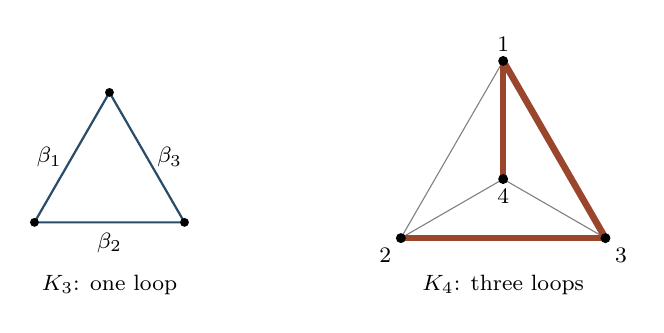
\begin{tikzpicture}[line cap=round]
  % K3
  \begin{scope}
    \coordinate (a) at (90:1.1); \coordinate (b) at (210:1.1); \coordinate (c) at (330:1.1);
    \draw[thick,inkblue] (a) -- node[left,font=\footnotesize,black] {$\beta_1$} (b)
                               -- node[below,font=\footnotesize,black] {$\beta_2$} (c)
                               -- node[right,font=\footnotesize,black] {$\beta_3$} (a);
    \foreach \p in {a,b,c} \fill (\p) circle (1.6pt);
    \node[font=\footnotesize] at (0,-1.35) {$K_3$: one loop};
  \end{scope}
  % K4 drawn flat
  \begin{scope}[shift={(5,0)}]
    \coordinate (1) at (90:1.5); \coordinate (2) at (210:1.5); \coordinate (3) at (330:1.5); \coordinate (4) at (0,0);
    \draw[thin,gray] (1) -- (2); \draw[thin,gray] (2) -- (4); \draw[thin,gray] (3) -- (4);
    \draw[line width=2.4pt,rust] (1) -- (3); \draw[line width=2.4pt,rust] (1) -- (4); \draw[line width=2.4pt,rust] (2) -- (3);
    \foreach \p/\pos in {1/above,2/below left,3/below right,4/below}{\fill (\p) circle (1.8pt); \node[\pos,font=\footnotesize] at (\p) {$\p$};}
    \node[font=\footnotesize] at (0,-1.35) {$K_4$: three loops};
  \end{scope}
\end{tikzpicture}

\caption{Left: the triangle $K_3$; its three spanning trees each leave out one edge, so
$U=\beta_1+\beta_2+\beta_3$. Right: the tetrahedron $K_4$ drawn flat, as a vacuum Feynman diagram with
four vertices, six lines and three loops. One of its $16$ spanning trees is drawn heavy; the three edges
left out give the monomial $\beta_{12}\beta_{34}\beta_{24}$ of $U$.}
\label{fig:k4}
\end{figure}

\paragraph{The triangle again.} For $n=2$ there are $N=3$ edges, every spanning tree leaves out exactly
one edge, and $U(\beta)=\beta_1+\beta_2+\beta_3$. The power $(n-2)/2$ is $0$, so~\eqref{eq:main} reads
\[
p_2=\frac1{\sqrt\pi}\int_{\R_+^3}\frac{e^{-(\beta_1+\beta_2+\beta_3)}}{(\beta_1+\beta_2+\beta_3)^{3/2}}\,\dd\beta
=\frac1{\sqrt\pi}\int_0^\infty\frac{s^2}{2}\,s^{-3/2}e^{-s}\,\dd s=\frac{\Gamma(3/2)}{2\sqrt\pi}=\frac14,
\]
grouping the $\beta$ by their sum $s$ (the set $\beta_1+\beta_2+\beta_3=s$ has area element $s^2/2$). The
long road through Gram matrices and spanning trees ends where the short argument of Section~1 did.

\paragraph{The simplex form.} The integrand of~\eqref{eq:main} without the exponential is homogeneous of
degree $N(n-2)/2-(N-n)(n+1)/2=-N/2$. Grouping $\beta$ by its sum in the same way gives
\begin{equation}\label{eq:simplex}
p_n=C_n\,\Gamma(N/2)\int_{\Delta}\frac{\prod_e\sigma_e^{(n-2)/2}}{U(\sigma)^{(n+1)/2}}\,\dd\sigma,
\end{equation}
over the simplex $\Delta=\{\sigma_e\ge0,\ \sum\sigma_e=1\}$ with its Lebesgue measure of total mass
$1/(N-1)!$. This is the form used for computing.

\section{The tetrahedron as a Feynman diagram}\label{sec:feynman}

In a Euclidean quantum field theory with one particle of mass $1$, a vacuum diagram is a graph whose lines
carry momenta $q_e\in\R^D$, conserved at each vertex, so that the free momenta are one $k\in\R^D$ per
independent loop. A line with propagator power $\nu$ contributes $(q_e^2+1)^{-\nu}$. Writing each factor as
$\Gamma(\nu)^{-1}\int_0^\infty\alpha^{\nu-1}e^{-\alpha(q_e^2+1)}\dd\alpha$ and doing the Gaussian integral over
the loop momenta gives the standard parametric representation~\cite[eqs.~(7)--(9) and Section~4]{BW10}:
\[
\int\prod_{\text{loops}}\frac{\dd^Dk}{\pi^{D/2}}\prod_e\frac1{(q_e^2+1)^{\nu}}
=\frac1{\Gamma(\nu)^N}\int_{\R_+^N}\frac{\prod_e\alpha_e^{\nu-1}e^{-\sum\alpha_e}}{U(\alpha)^{D/2}}\,\dd\alpha,
\]
with the same $U$, the sum over spanning trees of the products of the omitted variables. Comparing with
Theorem~\ref{thm:main}: $\nu-1=(n-2)/2$ and $D/2=(n+1)/2$.

\begin{corollary}\label{cor:feynman}
$p_n=C_n\,\Gamma(n/2)^N\,T_n$, where $T_n$ is the vacuum diagram of the complete graph $K_{n+1}$ in
dimension $D=n+1$, with all masses $1$ and every propagator raised to the power $n/2$.
\end{corollary}

\begin{table}[ht]
\centering
\begin{tabular}{cccccl}
\toprule
$n$ & lines $N$ & loops $N-n$ & dimension $D$ & power $\nu$ & $p_n$\\
\midrule
$2$ & $3$ & $1$ & $3$ & $1$ & $1/4$\\
$3$ & $6$ & $3$ & $4$ & $3/2$ & $0.0125749944\ldots$\\
$4$ & $10$ & $6$ & $5$ & $2$ & $1.0584\times10^{-4}$ (Monte Carlo)\\
\bottomrule
\end{tabular}
\caption{The diagram behind each $p_n$. For the triangle, $T_2=\int\dd^3k/\pi^{3/2}\,(k^2+1)^{-3}=
\Gamma(3/2)/\Gamma(3)=\sqrt\pi/4$ and $C_2=1/\sqrt\pi$, so $p_2=1/4$ once more.}
\label{tab:diagrams}
\end{table}

For the tetrahedron, $C_3\Gamma(3/2)^6=(4/\pi)(\pi^3/64)=\pi^2/16$, which is the formula $p_3=\pi^2T/16$ of the
introduction. Table~\ref{tab:diagrams} lists the first three cases. The tetrahedron diagram with equal
masses has a long history in particle physics, where it appears at three loops. With every power equal
to $1$ in four dimensions, and masses $0$ or $1$, Broadhurst reduced its finite part to a few constants built
from the sixth root of unity, such as $\zeta(3)$ and the Clausen value $\mathrm{Cl}_2(\pi/3)$~\cite{Bro99}.
The power $3/2$ that the broken stick asks for is not among the cases treated there, and we have found no
evaluation of it.

\section{Numbers}\label{sec:numbers}

\paragraph{The tetrahedron.} Two computations that share only the reduction to exponential lengths give
\[
p_3=0.0125749944167\ldots,
\]
agreeing to within $10^{-12}$.

The first works in the lengths. Hold the two faces that meet along edge $12$ and rotate one about that
edge, as in Figure~\ref{fig:hinge}. The opposite edge $34$ then takes every length between its values in
the two flat positions, and no others, so the sixth exponential length can be integrated out exactly. Scaling
out the length of edge $12$ leaves a four-dimensional integral over the positions of the two apexes.
In elliptic coordinates its integrand is smooth except where the two apexes project to the same point, and
polar coordinates centred there with Gauss quadrature give $0.0125749944167$; raising the inner order from
$24$ to $40$ and the outer from $16$ to $24$ moves the result by less than $10^{-13}$.

\begin{figure}[ht]
\centering
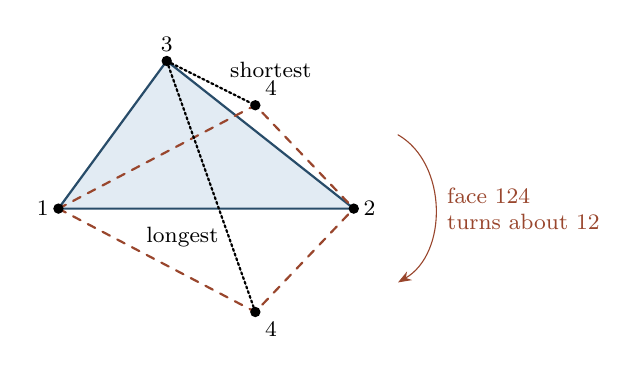
\begin{tikzpicture}[scale=1.25,line cap=round]
  \coordinate (1) at (0,0); \coordinate (2) at (3,0); \coordinate (3) at (1.1,1.5);
  \coordinate (4u) at (2.0,1.05); \coordinate (4d) at (2.0,-1.05);
  \fill[softblue] (1) -- (2) -- (3) -- cycle;
  \draw[thick,inkblue] (1) -- (2) -- (3) -- cycle;
  \draw[thick,rust,dashed] (1) -- (4u) -- (2); \draw[thick,rust,dashed] (1) -- (4d) -- (2);
  \draw[->,>=Stealth,rust] (3.45,0.75) to[bend left=60] (3.45,-0.75);
  \node[right,font=\footnotesize,rust,align=left] at (3.85,0) {face $124$\\turns about $12$};
  \draw[densely dotted,thick] (3) -- node[above right,font=\footnotesize,pos=0.6] {shortest} (4u);
  \draw[densely dotted,thick] (3) -- node[left,font=\footnotesize,pos=0.7] {longest} (4d);
  \foreach \p/\lab/\pos in {1/1/left,2/2/right,3/3/above,4u/4/above right,4d/4/below right}{\fill (\p) circle (1.5pt); \node[\pos,font=\footnotesize] at (\p) {$\lab$};}
\end{tikzpicture}

\caption{Two faces hinged on edge $12$. As the face $124$ turns, the length $\abs{x_3x_4}$ runs over an
interval whose ends are the two flat positions (dashed). A tetrahedron exists exactly when the sixth length
lies inside this interval.}
\label{fig:hinge}
\end{figure}

The second integrates the simplex form~\eqref{eq:simplex} with $n=3$. Splitting $\Delta$ into six sectors
according to its largest coordinate and putting $\sigma=s^2$ in the others removes every singularity, and
product Gauss rules of orders $24,28,\dots,44$ give $0.0125749944383$, $\ldots44216$, $\ldots44180$,
$\ldots44171$, $\ldots44168$, $\ldots44168$, settling on the same value from above.

A plain Monte Carlo simulation of the original question, testing the Cayley--Menger condition for
$3\times10^8$ random sticks, gives $0.012576\pm0.000006$. The value $1/79=0.0126582$ reported
in~\cite{MO} is $0.66\%$ too high, which is $13$ standard errors of that simulation. Against Zare's
polytope, of volume $1/54$, the Cayley--Menger condition keeps $54p_3\approx 68\%$.

\paragraph{The $4$-simplex.} Monte Carlo on both sides of Theorem~\ref{thm:main} for $n=2,3,4$, with
$2\times10^7$ samples each, agrees within one standard error in every case. For $n=4$ the integral side
gives $p_4=1.0584\times10^{-4}$ with standard error $2\times10^{-8}$, and the direct simulation of ten
exponential lengths gives $(1.069\pm0.023)\times10^{-4}$.

\paragraph{Any order.} The question as Dickman asked it~\cite{MO} lets the six pieces be placed on the
edges in whichever order works. Up to the symmetries of the tetrahedron there are $30$ essentially
different orders, and the event is the union of their $30$ events. Randomised quasi-Monte Carlo over this
union gives $0.0652818\pm0.0000004$, in agreement with the estimate $0.0652823\pm0.0000113$ by Sasha on
Mathematics Stack Exchange~\cite{MSE}.

\section{What is left}\label{sec:left}

No closed form is known for $p_3$ or for the unordered probability. Searches for integer relations with
three or four terms and coefficients up to $200$, between $p_3$ (to eleven digits) and constants such as
$\pi$, $\pi^2$, $\zeta(3)$, $\log 2$, $\log 3$, $\sqrt2$, $\sqrt3$, Catalan's constant and
$\mathrm{Cl}_2(\pi/3)$, found none. That is
weak evidence at this precision. Theorem~\ref{thm:main} at least places the problem: a closed form for
$p_3$ is a closed form for an equal-mass three-loop diagram with half-integer powers, and the methods that
evaluate such diagrams~\cite{Bro99,BW10} are the natural tools. The unordered probability is a union of $30$
such events and is unlikely to be simpler.

\paragraph{Verification.} The algebra behind Theorem~\ref{thm:main} for the triangle and the tetrahedron
is checked in Lean~4 with Mathlib~\cite{mathlib}, using only the standard axioms: the map~\eqref{eq:gram}
and its determinant, identity~\eqref{eq:trace}, the count of $16$ spanning trees of $K_4$, the matrix-tree
expansion of $\det L_t$ for $K_3$ and $K_4$, the duality~\eqref{eq:dual}, the substitution
$t_e=1/(4\beta_e)$, the homogeneity degree, the constants $C_2=1/\sqrt\pi$, $C_3=4/\pi$ and
$C_3\Gamma(3/2)^6=\pi^2/16$, and $p_2=1/4$. The analytic inputs (the exponential representation of a broken
stick, Schoenberg's criterion, Lemma~\ref{lem:schwinger} and Siegel's integral) are quoted. Python programs
compute $p_3$ by the two methods of Section~\ref{sec:numbers}, test Theorem~\ref{thm:main} by Monte Carlo for
$n=2,3,4$, and assert every number stated here; deliberately wrong variants of the programs fail those
checks. A C program computes the unordered probability. An independent program, sharing no code with the
others, rechecks the values, Zare's $1/54$, and the unordered probability over all $720$ orders.
Everything is at \url{https://github.com/jvvk/mathematics/tree/main/broken-stick-feynman}.

\paragraph{Acknowledgements.} Benjamin Dickman asked the question; Douglas Zare, Kirill and Sasha
contributed the polytope bound and the earlier numbers. Anthropic's Claude (Opus~5.5) was used to find the
arguments, write the Lean formalisation and the programs, and draft this text. The author takes
responsibility for the content.

\begin{thebibliography}{99}
\bibitem{MO} B.~Dickman, Probability that a stick randomly broken in five places can form a tetrahedron,
MathOverflow question 142983 (2013), \url{https://mathoverflow.net/q/142983}, accessed 10 October 2026.
\bibitem{Zare} D.~Zare, answer to~\cite{MO}, \url{https://mathoverflow.net/a/153783} (2014), accessed
10 October 2026.
\bibitem{MSE} B.~Dickman, Probability that a stick randomly broken in five places can form a tetrahedron,
Mathematics Stack Exchange question 351913 (2013), with the answer by Sasha,
\url{https://math.stackexchange.com/a/370750}, accessed 10 October 2026.
\bibitem{AGJMPV} T.~Amdeberhan, M.~L.~Glasser, M.~C.~Jones, V.~H.~Moll, R.~Posey and D.~Varela, The
Cauchy--Schl\"omilch transformation, arXiv:1004.2445 (2010).
\bibitem{BW10} C.~Bogner and S.~Weinzierl, Feynman graph polynomials, \emph{Internat. J. Modern Phys. A}
\textbf{25} (2010) 2585--2618,
\href{https://doi.org/10.1142/S0217751X10049438}{doi:10.1142/S0217751X10049438}.
\bibitem{Bro99} D.~J.~Broadhurst, Massive 3-loop Feynman diagrams reducible to SC$^*$ primitives of
algebras of the sixth root of unity, \emph{Eur. Phys. J. C} \textbf{8} (1999) 311--333,
arXiv:hep-th/9803091.
\bibitem{Dev86} L.~Devroye, \emph{Non-Uniform Random Variate Generation}, Springer, New York, 1986.
\bibitem{IP10} E.~J.~Ionascu and G.~Prajitura, Things to do with a broken stick, arXiv:1009.0890 (2010).
\bibitem{Kir1847} G.~Kirchhoff, Ueber die Aufl\"osung der Gleichungen, auf welche man bei der Untersuchung
der linearen Vertheilung galvanischer Str\"ome gef\"uhrt wird, \emph{Ann. Phys.} \textbf{148} (1847)
497--508, \href{https://doi.org/10.1002/andp.18471481202}{doi:10.1002/andp.18471481202}.
\bibitem{LLMM14} L.~Liberti, C.~Lavor, N.~Maculan and A.~Mucherino, Euclidean distance geometry and
applications, \emph{SIAM Rev.} \textbf{56} (2014) 3--69,
\href{https://doi.org/10.1137/120875909}{doi:10.1137/120875909}.
\bibitem{Mui82} R.~J.~Muirhead, \emph{Aspects of Multivariate Statistical Theory}, Wiley, New York, 1982.
\bibitem{Sch35} I.~J.~Schoenberg, Remarks to Maurice Fr\'echet's article ``Sur la d\'efinition
axiomatique d'une classe d'espace distanci\'es vectoriellement applicable sur l'espace de Hilbert'',
\emph{Ann. of Math.} (2) \textbf{36} (1935) 724--732,
\href{https://doi.org/10.2307/1968654}{doi:10.2307/1968654}.
\bibitem{Ver22} W.~Verreault, On the probability of forming polygons from a broken stick, \emph{Statist.
Probab. Lett.} \textbf{180} (2022) 109237,
\href{https://doi.org/10.1016/j.spl.2021.109237}{doi:10.1016/j.spl.2021.109237}.
\bibitem{mathlib} The mathlib Community, The Lean mathematical library, in \emph{Proceedings of the
9th ACM SIGPLAN International Conference on Certified Programs and Proofs (CPP 2020)}, 367--381,
\href{https://doi.org/10.1145/3372885.3373824}{doi:10.1145/3372885.3373824}.
\end{thebibliography}

\bigskip
\noindent Vamshi Jandhyala, London, UK.

\end{document}
